\documentclass[10pt,a4paper]{ltjsarticle}

\usepackage{graphicx}
\usepackage{amsmath,amssymb}
\usepackage{booktabs,subfig}
\usepackage{pifont}
\usepackage{url}
\usepackage{cite}
\usepackage{ulem}
\usepackage{siunitx}
\usepackage{float}
\usepackage{tcolorbox}
\usepackage{cancel}
\usepackage{color}
\renewcommand{\CancelColor}{\color{red}}

\usepackage{tikz}
\usepackage{circuitikz}
\usetikzlibrary{shadows}
\usetikzlibrary{calc}

\usepackage{luatexja-fontspec}
%\setmainfont[Ligatures=TeX]{TeXGyreTermes}
%\setsansfont[Ligatures=TeX]{TeXGyreHeros}
\setmainfont{TimesNewRoman}
\setsansfont{Arial}
\defaultjfontfeatures{Scale=1.0}
\setmainjfont[BoldFont=IPAexGothic]{IPAexMincho}
%\setmainjfont[BoldFont=HiraMinProN-W6]{HiraMinProN-W3}
%\setmainjfont[BoldFont=IPAexGothic]{KozMinPr6N-Light}
%\setmainjfont[BoldFont=IPAexGothic]{MS-PMincho}
\setsansjfont{IPAexGothic}
%\setsansjfont{MS-PGothic}
%\setsansjfont[BoldFont=HiraginoSans-W8]{HiraginoSans-W4}

%\renewcommand{\figurename}{Fig.~}
\renewcommand{\figurename}{Figure~}
\renewcommand{\tablename}{Table~}

\begin{document}
\title{シンクロトロン振動のほへと}
\author{吉本伸一}
\maketitle
\tableofcontents
\clearpage

\section{はじめに}
シンクロトロン蓄積リングでは、偏向電磁石によって分散 (dispersion) が発生する為、粒子の横方向と縦方向の運動が結合する。この結合が、リングを周回する粒子の縦方向の振動 (シンクロトロン振動) において重要な役割を演じる。
%シンクロトロン振動は基準粒子(設計軌道を設計速度で運動する粒子)に対する、到着時間と運動量偏差の振動である。

\section{Synchronous particle}
運動量$p_0$を持つ粒子が、基準軌道\footnote{粒子の運動量に対応して、一定の閉じた軌道 (閉軌道) が存在する。}\ を周期$T_0$で周回し、高周波加速空洞を同じ位相$\phi_s$で通過する時、このような粒子のことを同期粒子 (synchronous particle) と呼ぶ。同期粒子であるためには、周回周波数$f_0 (= 1/T_0)$と空洞のRF周波数$f_{RF}$の間に
%
\begin{equation}
    f_{RF} = h f_0
    \label{harmonic}
\end{equation}
%
という関係が必要である。整数$h$をharmonic numberと言い、周波数$f_{RF}$で加速できる最大の粒子数になる。この時、空洞の加速電圧は
%
\begin{equation}
    V_c (\phi) = V_0 \sin (\phi),\:\phi = \omega_{RF} t + \phi_s
\end{equation}
%
となる。図\ref{synchronous}は、$h=2$の時の空洞電圧と同期粒子の関係を表してる。

\begin{figure}[hbt]
    \begin{center}
      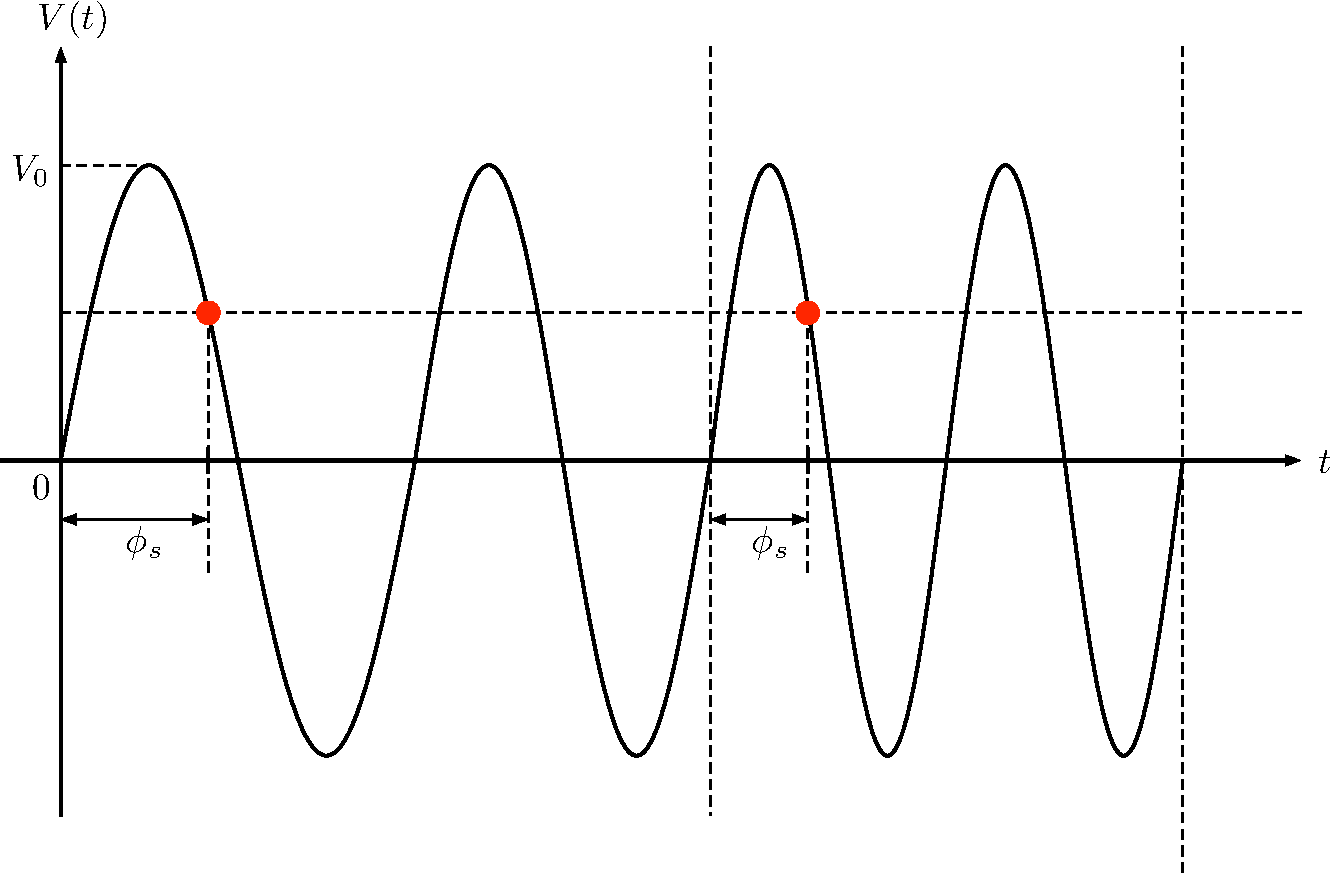
\includegraphics[width=15cm,clip]{synchronous.pdf}
      \caption{$f_{RF} = h f_0$ ($h=2$)}
      \label{synchronous}
    \end{center}
\end{figure}

\begin{tcolorbox}[title=\textgt{SuperKEKBにおける$f_{RF}$, $f_{0}$, $h$}の関係]
    SuperKEKBのリングでは、電子と陽電子は、ほぼ光速$c$で回っており、周長$C_0$は$\SI{3016.315}{\meter}$なので周回周波数$f_0$は
    %
    \begin{equation}
      f_0 = \frac{1}{T_0}=\frac{c}{C_0}=\frac{\SI{2.99792458e8}{\meter / \second}}{\SI{3016.315}{\meter}}=\SI{99.39}{\kilo\hertz} \notag
    \end{equation}
    %
    一方、RF周波数$f_{RF}$は$\SI{508.887}{\mega\hertz}$なので
    %
    \begin{equation}
        f_{RF} = 5120 f_0 \notag
    \end{equation}
    となり、確かに(\ref{harmonic})を満たしている。
\end{tcolorbox}

\section{Dispersion effects in a synchrotron}
粒子の運動量が変化すると、速度や軌道長も変わる。今、運動量偏差 (momentum deviation) を
%
\begin{equation}
    \delta_p = \frac{p-p_0}{p_0}=\frac{\Delta p}{p_0}
\end{equation}
%
とし、同期粒子より運動量が大きい粒子 ($\delta_p >0$) が偏光磁石を通過する場合を考える (Figure~\ref{dispersion})。
%
\begin{figure}[hbt]
    \begin{center}
      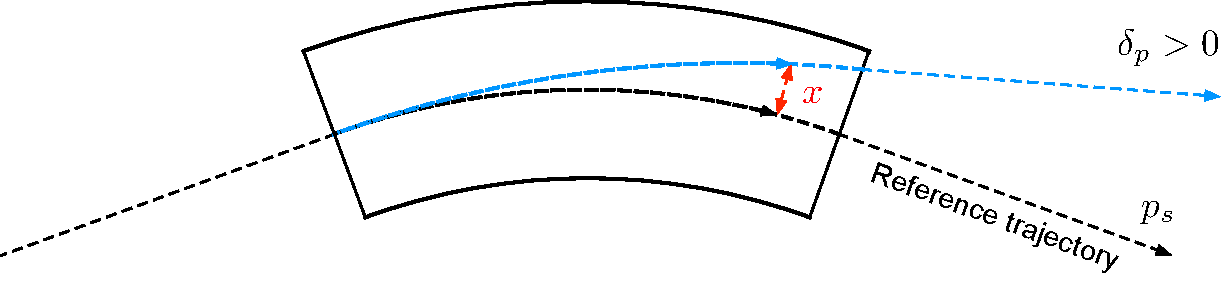
\includegraphics[width=15cm,clip]{dispersion.pdf}
      \caption{Change in path length for a particle in a dipole magnet (with bending radius $\rho$) resulting from the horizontal displacement of the particle from the reference trajectory.}
      \label{dispersion}
    \end{center}
\end{figure}
%
その粒子は曲げられにくい為、基準軌道とは異なる軌道を通ることになる。この軌道のずれ$x(s)$は分散関数 (dispersion function) $D_x(s)$を用いて、
%
\begin{equation}
    x(s) = D_x(s)\frac{\Delta p}{p_0} = D_x(s)\delta_p 
\end{equation}
%
と表される。今、基準軌道の曲率半径を$\rho$とすると$ds = \rho d\theta$より、
%
\begin{equation}
    dC = (\rho + x) d\theta = (\rho + x) \frac{ds}{\rho}
\end{equation}
%
したがって、この粒子の軌道長 $C$ は、
%
\begin{align}
    C &= \oint (\rho + x)\frac{ds}{\rho} = \int_0^{C_0} ds + \int_0^{C_0}\frac{x}{\rho} ds \notag \\
    &= C_0 + \delta_p \int_0^{C_0}\frac{D_x(s)}{\rho} ds
\end{align}
%
ここで運動量圧縮率 (momentum compaction factor) $\alpha_p$ を
%
\begin{equation}
    \alpha_p \equiv \frac{1}{C_0} \oint \frac{D(s)}{\rho} ds
\end{equation}
%
と定義すると、軌道長の差 $\Delta C = C-C_0$ は、
%
\begin{equation}
    \frac{\Delta C}{C_0}=\alpha_p\frac{\Delta p}{p_0}=\alpha_p\delta_p
    \label{delta_C}
\end{equation}
%
となり$\alpha_p$は運動量の変化による相対的な軌道長の変化を表していることになる。

次に、運動量の変化が回転周期に及ぼす影響を考える事にする。運動量の変化$\Delta p$によって、速度と回転周期がそれぞれ $v=v_0+\Delta v$ と $T=T_0+\Delta T$ に変化した時、回転周期は $T=C/v$ であるので、
%
\begin{equation}
    \frac{\Delta T}{T_0} = \frac{\Delta C}{C_0} - \frac{\Delta v}{v_0}
    \label{delta_T}
\end{equation}
%
となる。この式より、回転周期の変化 ($\Delta T/T_0$) をもたらす要因として、軌道長の変化 ($\Delta C/C_0$) と粒子の速度の変化 ($\Delta v/v_0$)である事が分かる。ここで(\ref{dv_dp}) より
%
\begin{equation}
    \frac{\Delta v}{v_0}=\frac{1}{\gamma_0^2}\frac{\Delta p}{p_0}
    \label{delta_v}
\end{equation}
%
(\ref{delta_T}) に (\ref{delta_C}) と (\ref{delta_v})を代入すると、
%
\begin{equation}
    \frac{\Delta T}{T_0} = \left(\alpha_p - \frac{1}{\gamma_0^2}\right)\frac{\Delta p}{p_0} = \eta_p \delta_p
\end{equation}
%
ただし、
%
\begin{equation}
    \eta_p \equiv \alpha_p - \frac{1}{\gamma_0^2} = \frac{1}{\gamma_t^2} - \frac{1}{\gamma_0^2}
    \label{alppha_slip}
\end{equation}
%
はphase slip factorと言い、運動量の変化による相対的な回転周期$T$の変化率を表している。
%

運動量圧縮率が正の場合 ($\alpha_p>0$) を考える。このとき、粒子の運動量を増加させると経路長が増加する。 しかし、粒子の運動量がまだ低く、光度よりも十分遅い場合、粒子の運動量の増加による速度の増加は、運動量の増加による経路長の増加を越えることがあり得る。その結果、粒子の回転周期は短くなる ($\eta_p < 0$)。
一方、粒子の運動量が十分高く超相対論的粒子の場合、粒子の速度は既に光速に十分近く、運動量の増加による速度の増加は極僅かである。この場合、経路長の増加が速度の増加を上回り、粒子の回転周期は長くなる ($\eta_p>0$) 。$\eta_p = 0$の時、つまり
%
\begin{equation}
    \gamma_t = \frac{1}{\sqrt{\alpha_p}}
\end{equation}
%
では回転周期は運動量に依存しない。この$\gamma_t$を遷移エネルギー (transition energy) と言う。

\vspace{\baselineskip}

\begin{tcolorbox}[title=式 (\ref{delta_T}) の導出]
    $v = v_0 + \Delta v$, $C=C_0 + \Delta C$, $T = T_0 + \Delta T$ とすると $T = C/v$ より、
    \begin{equation}
        T_0 + \Delta T = \frac{C_0 + \Delta C}{v_0 + \Delta v} \notag
    \end{equation}
    %
    分母を払って整理すると、(二次の微小量は無視する)
    %
    \begin{align}
        & (T_0 + \Delta T)(v_0 + \Delta v) = C_0 + \Delta C \notag \\
        \Longleftrightarrow\quad & \underset{C_0}{\uwave{\cancel{v_0 T_0}}} + \Delta v T_0 + v_0 \Delta T +
        \underset{0}{\uwave{\cancel{\Delta v \Delta T}}}
        = \cancel{C_0} + \Delta C \notag \\
        \Longleftrightarrow\quad & v_0 \Delta T = \Delta C- \Delta v T_0 \notag \\
        \Longleftrightarrow\quad & \frac{\Delta T}{T_0} = \frac{\Delta C_0}{\underset{C_0}{\uwave{v_0 T_0}}} - \frac{\Delta v}{v_0} \notag \\
        \Longleftrightarrow\quad & \frac{\Delta T}{T_0} = \frac{\Delta C_0}{C_0} - \frac{\Delta v}{v_0} \notag
    \end{align}
\end{tcolorbox}

%\clearpage

\section{Phase stability}
ビームの中には多くの粒子があり、色々な運動量を持つ粒子で構成されている。同期粒子と異なる運動量を持つ粒子が加速空洞を通過する時、どのように加速されるかについて考えてみる。
%
\begin{figure}[hbt]
    \begin{center}
      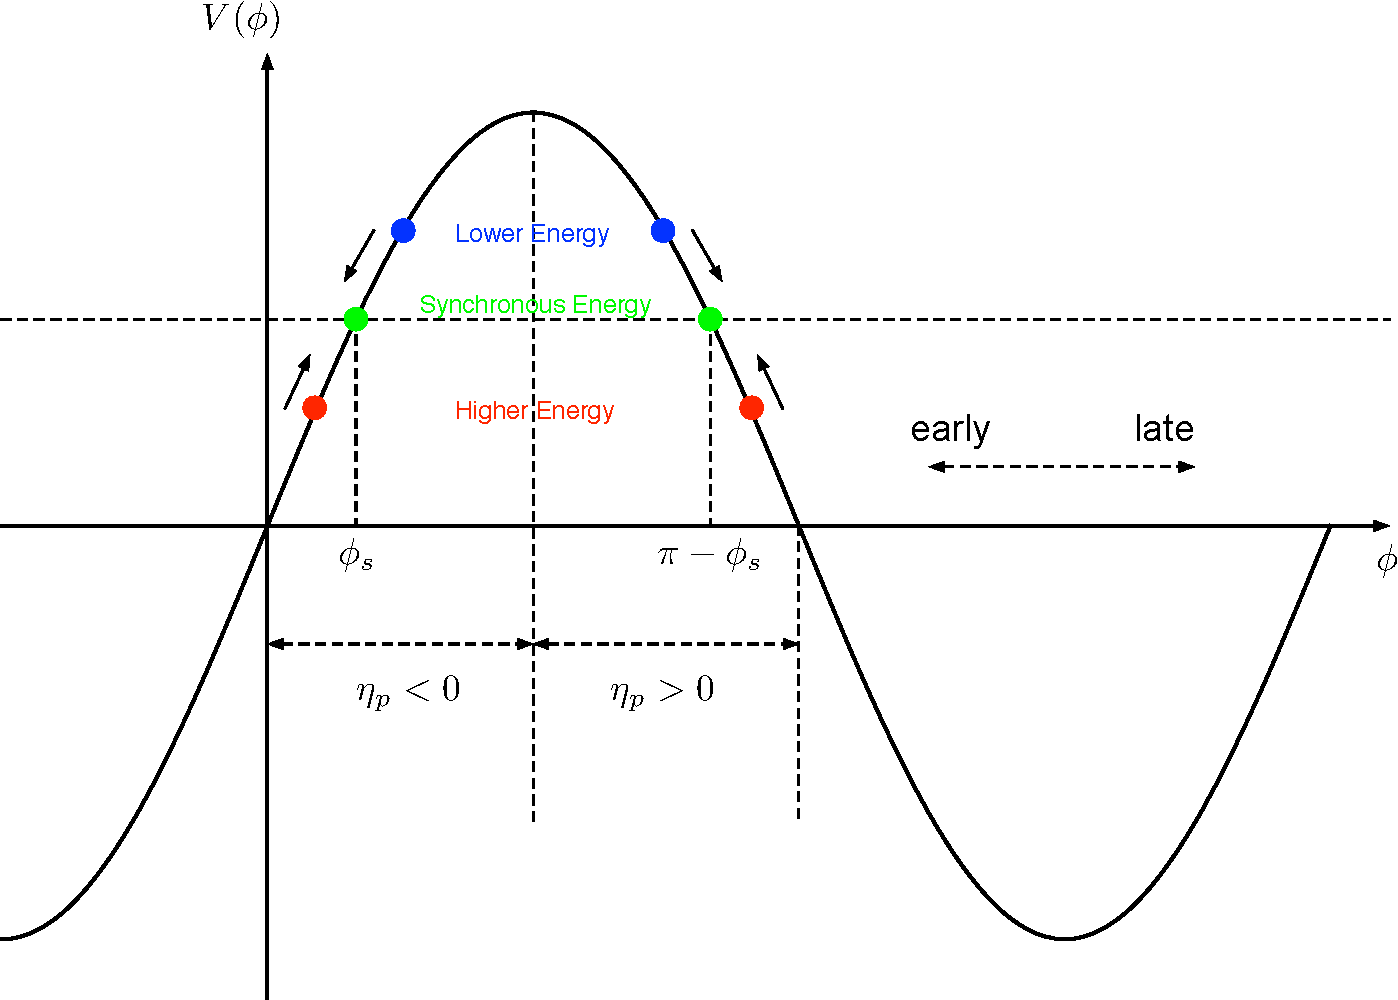
\includegraphics[width=15cm,clip]{phase_stability.pdf}
      \caption{Schematic drawing of an rf wave, and the rf phase angles for a synchronous, a higher, and a lower energy particles.
      For a stable synchrotron motion, the phase focusing principle requires $0 < \phi_s \leq \pi/2$ for $\eta_p < 0$,
      and $\pi/2 < \phi_s \leq \pi$ for $\eta_p > 0$.}
      \label{phase_stability}
    \end{center}
\end{figure}

$\eta_p < 0$ の時、同期粒子より大きい運動量を持つ粒子は、同期粒子より回転周期が短いので、同期粒子より早く加速空洞に到着する。したがって、同期位相$\phi_s$を$0<\phi_s<\pi/2$に選べば、より大きい運動量を持つ粒子は、同期粒子より少ないエネルギーを加速空洞から得ることになる。同様に、同期粒子より小さな運動量を持つ粒子は、同期粒子より遅く加速空洞に到達するので、同期粒子より多いエネルギーを加速空洞から得る。この過程を繰り返すことで、同期粒子の持つ運動量から外れた運動量を持つ粒子は同期粒子の周りを安定に運動することが分かる。$\eta_p > 0$ の時は、同期位相を$\pi/2<\phi_s<\pi$に選べば同様にこの運動は安定である。

\section{Difference Equations for Longitudinal Motion in a Synchrotron}
The relative time $\tau$ and the relative phase $\phi$ are measured with respect to the zero crossing of the gap voltage. 
%
\begin{equation}
    \tau(n+1) - \tau(n) = T(n+1) -T_0(n+1)
\end{equation}
%
\begin{figure}[hhbt]
    \begin{center}
      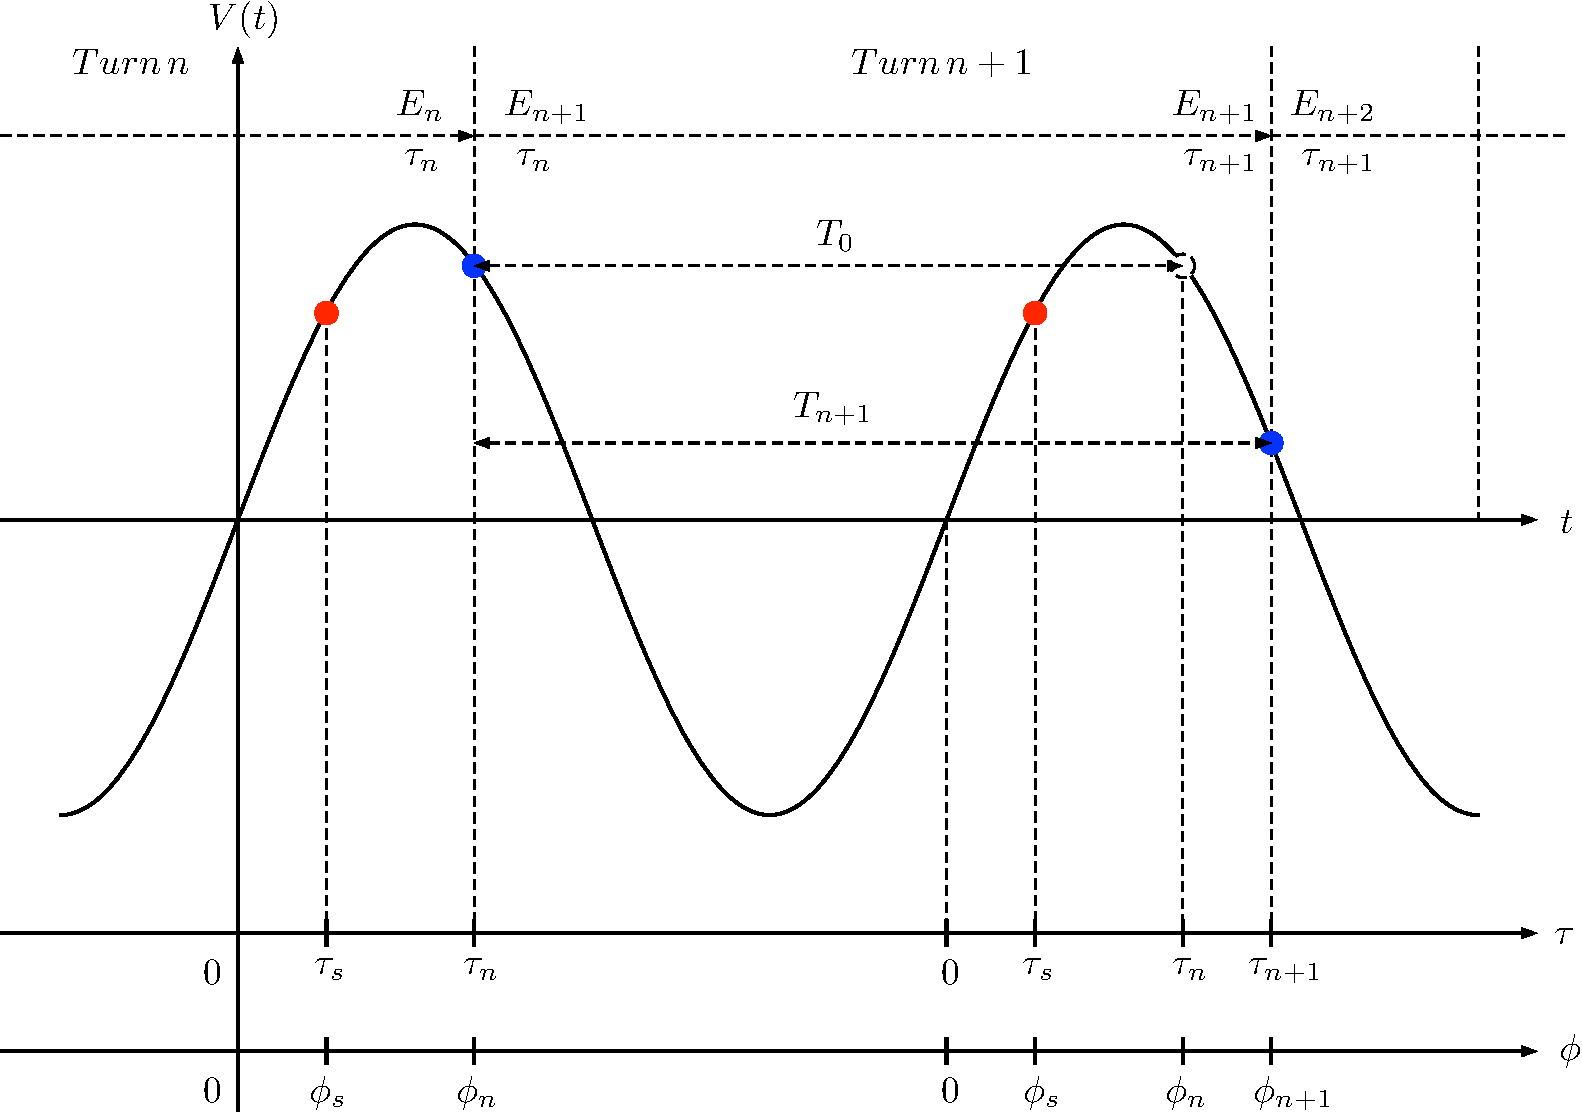
\includegraphics[width=15cm,clip]{coordinates.pdf}
      \caption{Relative and absolute coodinates. ($h=1$)}
      \label{coordinates}
    \end{center}
\end{figure}

$\phi(n) = \omega_{RF}(n) \tau(n)$と置くと
\begin{align}
    \phi(n+1) &= \omega_{RF}(n+1)\tau(n+1) \notag \\
    &=\omega_{RF}(n+1)\{\tau(n) + T(n+1) -T_0(n+1)\} \notag \\
    &= \frac{\omega_{RF}(n+1)}{\omega_{RF}(n)} \phi(n) + \omega_{RF}(n+1)\{T(n+1) -T_0(n+1)\}  \notag
\end{align}
%
ここで、
%
\begin{equation}
    \frac{T(n+1)-T_0(n+1)}{T_0(n+1)} = \eta \delta_p(n+1)
\end{equation}
%
\begin{align}
    \phi(n+1) &= \frac{\omega_{RF}(n+1)}{\omega_{RF}(n)}\phi(n) + \omega_{RF}(n+1)T_0(n+1)\eta \delta_p(n+1) \notag \\
    &=\frac{\omega_{RF}(n+1)}{\omega_{RF}(n)}\phi(n) + 2\pi h \eta \delta_p(n+1)
\end{align}
%
\begin{equation}
    \frac{\omega_{RF}(n+1)}{\omega_{RF}(n)}\phi(n) \approx 1
\end{equation}
%
\begin{equation}
    \phi(n+1) = \phi(n) + 2\pi h \eta \delta_p(n+1)
\end{equation}

The energy of a particle at the (n+1)-th turn $E(n+1)$ is expressed by the energy $E(n)$ and RF phase $\phi(n)$ at the n-th turn as
%
\begin{equation}
    E(n+1) = E(n) + e V \sin\phi (n)
\end{equation}
%
For a synchronous particle with suffix 0,
%
\begin{equation}
    E_0(n+1) = E_0(n) + e V \sin\phi_s
\end{equation}
%
Thus, the energy error, $\Delta E = E - E_0$, is expressed as
%
\begin{equation}
    \Delta E(n+1) = \Delta E(n) + e V (\sin\phi(n) - \sin\phi_s)
\end{equation}
%
ここで、
%
\begin{equation}
    \delta_p = \frac{\Delta p}{p_0} = \frac{1}{\beta_0^2}\frac{\Delta E}{E_0}
\end{equation}
%
より、
%
\begin{equation}
    \Delta E(n+1) - \Delta E(n) = \beta^2 E_0 \{\delta_p(n+1) - \delta_p(n)\}
\end{equation}
%
したがって、
%
\begin{equation}
    \delta_p(n+1) - \delta_p(n) = \frac{e V}{\beta_0^2 E_0}(\sin\phi(n) -\sin\phi_s)
\end{equation}
%

the symplectic mapping equation:
%
\begin{align}
    \begin{split}
        &\delta_p(n+1) - \delta_p(n) = \frac{e V}{\beta_0^2 E_0}(\sin\phi(n) -\sin\phi_s) \\
        &\phi(n+1) = \phi(n) + 2\pi h \eta \delta_p(n+1)
        \label{map}
    \end{split}
\end{align}
%

\section{Differential Equations for Longitudinal Motion in a Synchrotron}
The difference equations (\ref{map}) can be written as continuous differential equations, if the assumption is made that the change of the variables $\phi$ and $\delta_p$ during one turn in the ring is not too large. In this case, the difference quotient can be approximated by the differential quotient
%
\begin{equation}
    \frac{\delta_p(n+1)-\delta_p(n)}{T_0(n+1)} \approx \frac{d\delta_p}{dt}=\dot{\delta_p},\quad 
    \frac{\phi(n+1)-\phi(n)}{T_0(n+1)} \approx \frac{d\phi}{dt}= \dot{\phi}
\end{equation}
%
\begin{align}
    \begin{split}
        \dot{\delta_p} &= \frac{e V \omega_0}{2\pi \beta_0^2 E_0}(\sin\phi - \sin\phi_s) \\
        \dot{\phi} &= h \omega_0 \eta \delta_p
    \end{split}
\end{align}
%
\begin{equation}
    \ddot{\phi} = \frac{e V h \eta \omega_0^2}{2\pi\beta_0^2 E_0}(\sin\phi-\sin\phi_s)
\end{equation}
%
\subsection{Small amplitude approximation}
$\Delta\phi = \phi - \phi_s$が非常に小さい時、
%
\begin{equation}
    \sin\phi = \sin(\phi_s+\Delta\phi) \approx \sin\phi_s + \cos\phi_s \Delta\phi
\end{equation}
%
より
%
\begin{equation}
    \ddot{\Delta\phi} = \frac{e V h \eta \omega_0^2}{2\pi \beta_0^2 E_0} \cos\phi_s \Delta\phi = - \omega_s^2 \Delta\phi
\end{equation}
%
ただし、
%
\begin{equation}
    \omega_s = \sqrt{-\frac{e V h \eta \omega_0^2 \cos\phi_s}{2\pi \beta_0^2 E_0}}
\end{equation}
%

%
\subsection{$\delta$ and $\delta_p$}
Note that the momentum deviation $\delta_p$ is not the same as the energy deviation $\delta$. To proceed, it is useful to have a relationship between the derivative with respect to $\delta_p$ and the derivative with respect to $\delta$.
%
\subsubsection{energy deviation}
%
\begin{equation}
    \delta \equiv \frac{E}{P_0 c} -\frac{1}{\beta_0}
\end{equation}
%
$E =\gamma m c^2$, $P_0 =\beta_0\gamma_0 mc$より
%
\begin{align}
    \delta &= \frac{\gamma m c^2}{c(\beta_0\gamma_0 m c)} - \frac{1}{\beta_0} \notag \\
    & = \frac{1}{\beta_0}\left(\frac{\gamma}{\gamma_0} - 1\right) \notag \\
    & = \frac{1}{\beta_0}\left(\frac{E}{E_0}-1\right)
\end{align}
%
\subsubsection{momentum deviation}
%
\begin{equation}
    \delta_p = \frac{P}{P_0} -1
\end{equation}
%
Since $\delta_p = 0$ when $\delta = 0$, we can write:

\clearpage

\appendix
\renewcommand{\theequation}{\Alph{section}.\arabic{equation} }
\setcounter{equation}{0}

\section{相対論のおさらい}
\begin{equation}
    E_0 = m_0 c^2 ,\quad E = \sqrt{E_0^2 + p^2 c^2}
\end{equation}

\begin{equation}
    \beta = \frac{v}{c}\,,\quad \gamma = \frac{E}{E_0}=\frac{m}{m_0}=\frac{1}{\sqrt{1-\beta^2}}
\end{equation}

\begin{equation}
    p = mv = \gamma m_0 v = \gamma m_0 \beta c
\end{equation}

\begin{equation}
    \frac{p}{E} = \frac{\gamma m_0 \beta c}{\gamma m_0 c^2} = \frac{\beta}{c}
\end{equation}

式 (\ref{delta_v}) の導出

\begin{equation}
    \frac{dp}{dv} = m_0\frac{d}{dv}(\gamma v)
    = m_0 \left(\gamma + v \frac{d\gamma}{dv}\right) \notag
\end{equation}
%
\begin{align}
    \frac{d\gamma}{dv} & = \frac{1}{c}\frac{d\gamma}{d\beta}= \frac{1}{c}\frac{d}{d\beta}\left(\frac{1}{\sqrt{1-\beta^2}}\right) \notag \\
    & = \frac{1}{c} \beta \underset{\gamma^{-2}}{\underbrace{(1-\beta^2)}}^{-\frac{3}{2}} = \frac{\beta \gamma^3}{c} \notag \\
    & = \frac{1}{c} \beta \underset{\gamma^{-2}}{\uwave{(1-\beta^2)}}^{-\frac{3}{2}} = \frac{\beta \gamma^3}{c} \notag
\end{align}
%
これより、
\begin{align}
    \frac{dp}{dv} & = m_0 \left(\gamma + v \frac{\beta \gamma^3}{c}\right)
    = m_0 \gamma \underset{\gamma^2}{\uwave{(1 + \beta^2 \gamma^2)}}
    = \frac{\gamma^2 p}{v} \notag
\end{align}
%
\begin{equation}
    \therefore \quad \frac{dv}{v} = \frac{1}{\gamma^2}\frac{dp}{p}
    \label{dv_dp}
\end{equation}

\begin{align}
    p = mv = \gamma m_0 \beta c\,  , \quad E = \gamma E_0 = \gamma m_0 c^2 \notag
\end{align}
%
\begin{equation}
    \gamma \beta = \gamma \sqrt{1-\frac{1}{\gamma^2}} \notag = \sqrt{\gamma^2 -1} \notag
\end{equation}
%
\begin{align}
    \frac{dp}{dE} & = \frac{1}{c}\frac{d(\gamma \beta)}{d\gamma} = \frac{1}{c}\frac{d}{d\gamma}\sqrt{\gamma^2 -1} \notag \\
    & = \frac{\gamma}{c} \underset{\gamma^2\beta^2}{(\uwave{\gamma^2 -1}})^{-\frac{1}{2}} = \frac{1}{c\beta}
    = \frac{p}{\beta^2 E}\notag
\end{align}
%
\begin{equation}
    \therefore \quad \frac{dp}{p} = \frac{1}{\beta^2}\frac{dE}{E}
\end{equation}

\section{高周波加速空洞の基礎の基礎}
図~\ref{cavity1}はインダクタンス$L$とキャパシタンス$C$のよく知られた共振回路であり、この回路の共振周波数は、

\begin{equation}
  \omega = \frac{1}{\sqrt{LC}}
  \label{LC}
\end{equation}

で与えられる。いま、共振周波数が高いとき、(\ref{LC})より$L$と$C$は小さな値でもよく、極端な話、コイルの部分を引き伸ばして一本の線にした図~\ref{cavity2}のような回路でも共振回路として動作する。

\begin{figure}[hbt]
  \begin{center}
    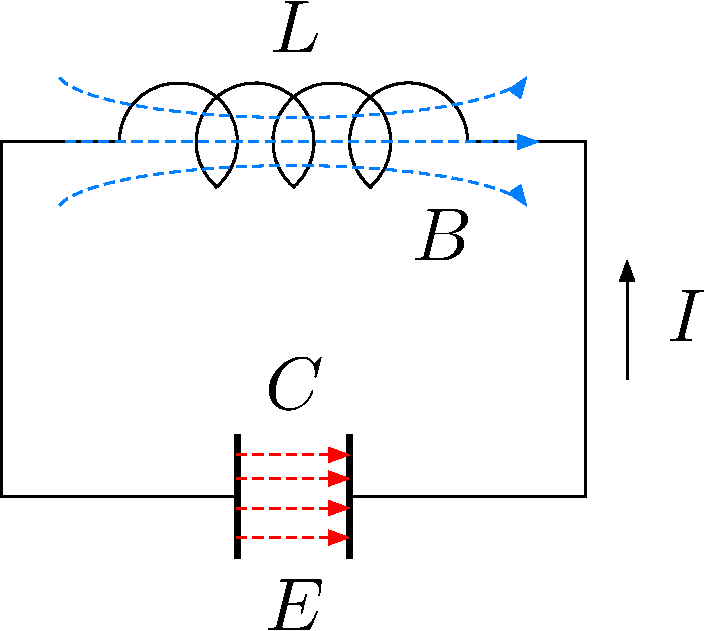
\includegraphics[width=8cm,clip]{cavity1.pdf}
    \caption{$LC$共振回路}
   \label{cavity1}
  \end{center}
\end{figure}

次に、この回路を$z$軸の周りに回転させると図~\ref{cavity3}のような金属の壁で囲まれたものが出来上がる。これも同様に共振回路として働き、空洞共振器と呼ばれる。空洞内では図に示すように。磁場は動径方向を周り、電場はギャップ部分に集中している。このギャップ部分に生じた高周波電場を使って荷電粒子を加速する装置が高周波加速空洞と言うことになる。

\begin{figure}[hbt]
  \begin{center}
    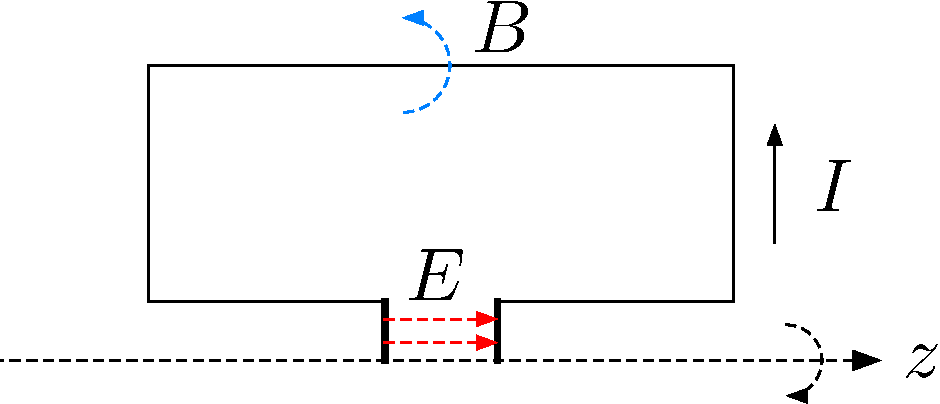
\includegraphics[width=8cm,clip]{cavity2.pdf}
    \caption{$LC$共振回路}
   \label{cavity2}
  \end{center}
\end{figure}

\begin{figure}[hbt]
  \begin{center}
    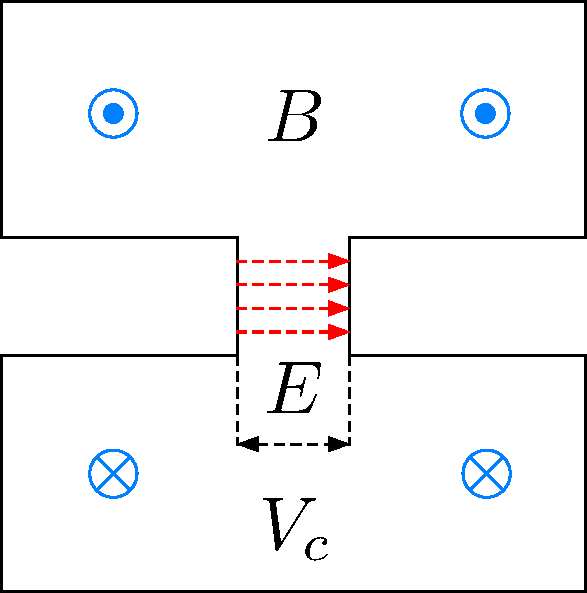
\includegraphics[width=6cm,clip]{cavity3.pdf}
    \caption{高周波加速空洞}
   \label{cavity3}
  \end{center}
\end{figure}

加速空洞の内面では、動径方向に走る磁場によって高周波電流が流れるので、空洞内面が持つ抵抗によって電力を損失する。したがって、共振状態を維持するためには外部より電力を供給する必要がある。いま、空洞の加速電圧を$V_{c}$、この電圧を維持するために必要な電力を$P_{c}$とすると、
%
\begin{equation}
  R_{sh} \equiv \frac{V_{c}^2}{P_{c}}
  \label{sh}
\end{equation}
%
で定義される量をシャントインピーダンスといい、空洞の特性を表す重要なパラメータの一つである。また、空洞内に蓄えられる電磁場のエネルギー$U$と空洞内の損失$P_{c}$を用いて、
%
\begin{equation}
  Q = \frac{\omega U}{P_{c}}
  \label{q_val}
\end{equation}
%
で表される量を空洞の$Q$値といい、これも空洞の特性を表す重要なパラメータとなっている。

\begin{tcolorbox}[title=\textgt{ARESとSCCの空洞損失}]
  ARESの場合、$Q_{0}=\num{1.33e5}$、$R_{sh}=\SI{1.7}{\mega \ohm}$で、空洞一台当たりの加速電圧を$V_{c}=\SI{0.5}{\mega\volt}$とすると、
%
\begin{equation*}
  P_{c} = \frac{V_{c}^2}{R_{sh}}=\SI{147}{\kilo \watt}
\end{equation*}

一方SCCの場合、$Q_{0}=\num{1e9}$、$R_{sh}=\SI{93e3}{\mega\ohm}$で、空洞一台当たりの加速電圧を$V_{c}=\SI{1.5}{\mega\volt}$とすると、
%
\begin{equation*}
  P_{c} = \frac{V_{c}^2}{R_{sh}}=\SI{24}{\watt}
\end{equation*}
%
となり、SCCの方が圧倒的に損失が少ない。(流石超電導!)
\end{tcolorbox}

\section{放射光によるエネルギー損失}
高エネルギーの荷電粒子が磁場によって曲げられる時、その進行方向に向かって電磁波を放射してエネルギーを失う。この現象のことをシンクロトロン放射と呼び、放射された電磁波を放射光という。シンクロトロン放射によって単位時間に放射されるエネルギーは、荷電粒子の質量の4乗に逆比例することが知られており、電子(陽電子)のように軽い粒子ほど放射されるエネルギーは大きくなる。実際、同じエネルギーを持つ電子と陽子が放射するエネルギーの比は、
%
\begin{equation}
  \frac{P_{p}}{P_{e}} = \left(\frac{m_e}{m_p}\right)=\left(\frac{9.1093897\times 10^{-31}\,\mathrm{kg}}{1.6726231\times 10^{-27}\,\mathrm{kg}}\right)=8.80\times 10^{-14}
  \label{eq4}
\end{equation}
%
となり。電子の方が圧倒的に多くのエネルギーを放射する。このように、シンクロトロン放射光によるエネルギー損失は、電子や陽電子のような非常に軽い粒子を加速するリングのみに現れてくる問題である。

詳しい計算によると

\section{静電場による繰り返し加速}
静電場を用いて荷電粒子を加速する場合、同じ加速電場を使って何度も繰り返し加速する事はできない。例えばFig.~\ref{dc_circular}のように磁場を使って荷電粒子を曲げ、何度も同じ電極を通過させた場合を考えてみる。粒子は電極を通る時に加速されるが、電極の外では逆に減速され加速した分が相殺されてしまう。このように、静電場を使って繰り返し加速はできないため、繰り返し加速を行う場合は、高周波電場を使うことになる。ただし、この図のように単純に平行平板の電極に高周波電圧を加えただけでは、静電場の時と同じように電極外で粒子が減速されてしまう場合がある。そこで、電磁場が外部に漏れないよう導体の壁によって囲まれた高周波加速空洞を使って繰り返し加速を行うことになる。
%
\begin{figure}[hbt]
  \begin{center}
    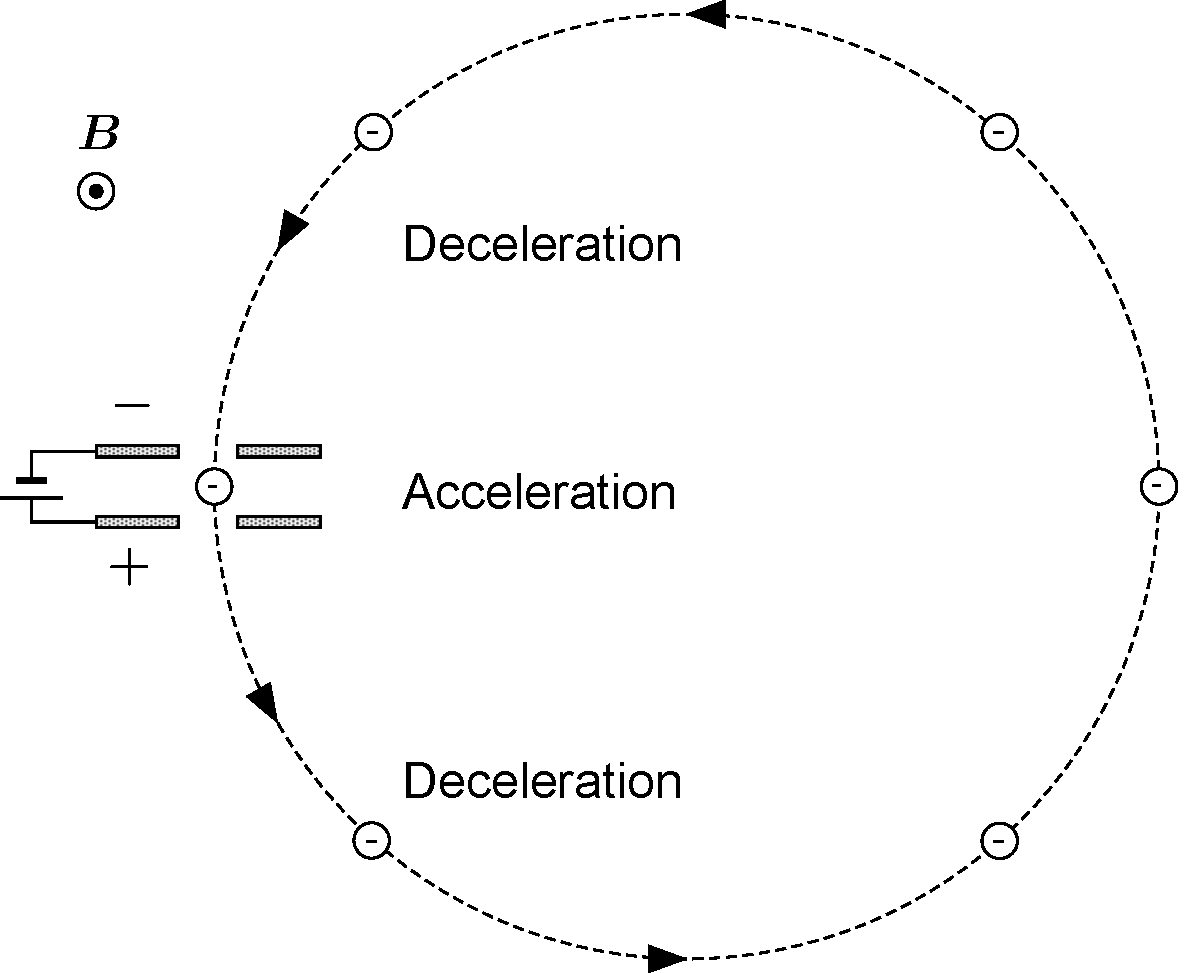
\includegraphics[width=10cm,clip]{dc_circular.pdf}
    \caption{静電場による繰り返し加速}
   \label{dc_circular}
  \end{center}
\end{figure}

\begin{thebibliography}{9}
    \bibitem{Chao}
    A. Chao, K. Mess, M. Tigner, and F. Zimmermann, Handbook of Accelerator Physics and Engineering (2nd Edition), World Scientific Publishing Company Incorporated, Singapore (2013)
    \bibitem{a}
    A.W.Chao and M.Tigner,editors.Handbook of Accelerator Physics and Engineering. World Scientific Pub. Co., 3rd printing edition, 2009.
    \bibitem{Wolski}
    Andy Wolski, Beam Dynamics in High Energy Particle Accelerators,  Imperial College Pr (2014).
    \bibitem{Lee}
    S. Y. Lee, Accelerator physics, World Scientific (2004), ISBN 9789812562005.
    \bibitem{Edwards}
    D.A. Edwards, M.J. Syphers, `An introduction to the physics of high energy accelerators', Wiley (1993).
\end{thebibliography}
%
\end{document}